\RequirePackage{plautopatch} % インポートしているパッケージに日本語対応の代替物があればそれをインポートするようにするコマンド(冒頭に書く)

% 論文誌のルールに従うように注意する。
% * ドキュメントクラスなど: 必ず論文誌が指定しているものを使う。
% * 句読点: 論文誌によって,「,」「。」であったり,「,」「.」あったりする。全角文字と半角文字の使い分けが要求されることもあるので注意。
% * タイトル,著者,日付など: 論文誌によって英文についても記載するようになっていたりと様々。
% * 文献の書き方: 論文誌によっては指定がある。

\documentclass[dvipdfmx]{jsarticle}
% \documentclass[dvipdfmx, twocolumn]{jsarticle} % 2段組みにする場合

\usepackage{graphicx} % 画像ファイルの取り込み \includegraphics コマンド
\usepackage{hyperref} % ハイパーリンク \href コマンド,\url コマンド

\begin{document}

% タイトル,著者,提出日付
\title{象の卵の重さと長径に関する考察}
\author{神谷年洋}
\date{2022年8月1日}
\maketitle

\section{はじめに}

この文書は,レポートや論文の書き方を示すためのサンプルです。
タイトルを「{象の卵の重さと長径に関する考察」としてあるのは,あえて荒唐無稽な内容とすることで,
間違えて修正せずに提出されてしまう\href{https://twitter.com/taku_ymnk/status/392959147974471681?s=20&t=3p7I92WEGvoPpj_7d-dtyA}{事故}を防ぐためです。 % URLのリンクを文書に埋め込む例
なお,本稿のタイトルを見て``d\'{e}j\`{a}vu''に襲われた方はおそらく研究者だと思われます。 % ダブルクオート、アクセントの利用例

象の卵の存在は現在も未確認であり,その外見については現在も想像するしかない。図\ref{fig:golden_egg}に,想像上の象の卵の外見を示す。 % 図の番号を参照する例

% 図の例
\begin{figure}[htp]
\centering
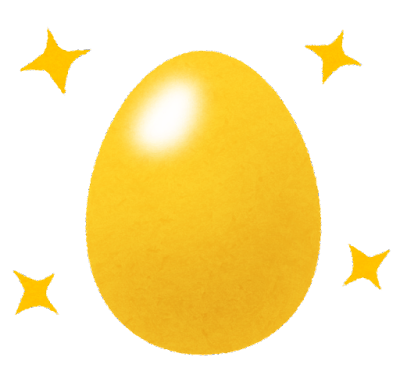
\includegraphics[width=3cm]{golden_egg.png}
\caption{象の卵の想像図}
\label{fig:golden_egg}
\end{figure}

\section{関連研究}
\label{sec:related} % 相互参照のラベルの例。節「関連研究」に「sec:related」というラベルをつけている

象の卵の味覚について,山中\cite{kakenhi_latex}は象の卵が美味しいと言われていることを指摘した。 % 文献の引用の例
象の卵の実在性に関する研究として,寺村ら\cite{teramura2009}は某国の王が実地に象の卵を捜索した事例を報告している。
過去日本にも大陸から象が渡ってきていることが指摘\cite{kamei1990}されており,象の卵が国内で発見される可能性も期待される。

\section{アプローチ}

象の卵を発見するためには,卵の重さやサイズが判明していることが望ましい。
\ref{sec:related}節の関連研究において象の卵が発見できていないのは,外見上の特徴がわからないために見逃している可能性がある。 % 相互参照の例
本稿では,他の動物との比較により,象の卵の重さやサイズが推定できるのではないかとのアイデアに基づく考察を行う。

\subsection{推定手法}

表\ref{tab:egg_sizes}に,他の動物と比較を示す。ゾウの卵の欄については,確認事例がないため空欄としている。
大雑把に,成体の体重と卵の重さが比例すると仮定し,さらに,重さの$\frac{1}{3}$乗が卵の長軸の長さに比例すると仮定することにより,象の卵の重さとサイズを推定する。

% 表の例
\begin{table}[htbp]
	\centering
	\caption{卵の大きさ}
  \label{tab:egg_sizes}
	\begin{tabular}{|c|r|r|r|}
		\hline
		動物 & 個体の重さ & 卵の重さ & 卵の長軸の長さ \\ \hline \hline
		ニワトリ & 4kg & 60g & 5.5cm \\ \hline
		ガチョウ & 9kg & 150g & 10cm \\ \hline
		ゾウ & 3t & ? & ? \\ \hline
	\end{tabular}
\end{table}

\begin{thebibliography}{99}
\bibitem{kakenhi_latex} 山中卓: 科研費LaTeX \url{https://osksn2.hep.sci.osaka-u.ac.jp/~taku/kakenhiLaTeX/} (2022年7月6日取得). % URLの引用
\bibitem{teramura2009} 寺村輝夫, 和歌山静子: ぼくは王様 - ぞうのたまごのたまごやき, 理論社, 2009年1月. % 書籍の引用
\bibitem{kamei1990} 亀井節夫: 日本海と象, 第四紀研究, 29巻, 3号, pp.~163--172, 2009-08-21. % 論文の引用
\end{thebibliography}

\end{document}
